\chapter{Diseño e implementación} % Main chapter title

\label{Chapter3}

En este capítulo se describen el diseño y la implementación del sistema de clasificación. En primer
lugar, se presentan la arquitectura general del sistema y las dos configuraciones que se
compararon. Luego, se describen el procesamiento de los datos, desde las grabaciones originales
hasta las ventanas que recibe el modelo, la arquitectura del modelo y su adaptación a la tarea, y
el procedimiento de entrenamiento. Por último, se explica cómo se obtiene el resultado de cada
grabación a partir de las predicciones del modelo.

%----------------------------------------------------------------------------------------

\section{Arquitectura del sistema}
\label{sec:arquitectura}

El sistema recibe una grabación de auscultación y determina si corresponde a un sonido cardíaco o
pulmonar y si presenta alguna de las alteraciones descritas en la sección \ref{sec:alteraciones}.
No es necesario indicarle el tipo de sonido ni el foco de auscultación, ya que ambos datos se
infieren a partir del audio. En esta sección se presentan las clases que distingue el sistema, las
etapas por las que pasa cada grabación y las dos configuraciones que se implementaron.

\subsection{Clases consideradas}
\label{subsec:clases}

Cada grabación se asigna a una de las siguientes seis clases:

\begin{itemize}
	\item Sonido cardíaco normal.
	\item Sonido cardíaco con soplo.
	\item Sonido pulmonar normal.
	\item Sonido pulmonar con crepitantes.
	\item Sonido pulmonar con sibilancias.
	\item Sonido pulmonar con crepitantes y sibilancias.
\end{itemize}

Los crepitantes finos y gruesos se agruparon en una misma clase. Los roncus se incluyeron en la
clase de sibilancias, ya que ambos son sonidos continuos. La última clase representa los casos en
los que las dos alteraciones aparecen de forma conjunta. Además, esta agrupación permite unificar
las etiquetas de las distintas bases de datos descritas en la sección \ref{sec:basesDatos}.

\subsection{Procesamiento de una grabación}
\label{subsec:procesamiento}

El procesamiento de una grabación sigue las etapas de la figura \ref{fig:arquitectura}a. Primero,
la señal se lleva a un formato común, con una misma frecuencia de muestreo y una amplitud
normalizada. Luego, se divide en ventanas de duración fija que se superponen parcialmente, y cada
ventana se transforma en un espectrograma log-Mel. El modelo asigna a cada ventana una probabilidad
para cada clase. Por último, las predicciones de todas las ventanas se combinan para obtener una
única decisión por grabación: primero el tipo de sonido y luego, dentro de ese tipo, la alteración.

Se optó por ventanas de duración fija por dos razones. Por un lado, las grabaciones tienen
duraciones distintas y las alteraciones pueden aparecer solo en una parte de ellas, como ocurre con
los crepitantes, que se concentran en la inspiración. Por otro lado, las ventanas fijas no
requieren segmentar la señal en ciclos cardíacos o respiratorios. Si bien algunas bases de datos
incluyen esa segmentación, no estaría disponible en el uso real del sistema. Además, las ventanas
con las que se entrena el modelo son las mismas que recibe al predecir, por lo que se lo evalúa en
las mismas condiciones en las que fue entrenado.

\subsection{Configuraciones integrada y separada}
\label{subsec:configuraciones}

Para comparar un enfoque integrado con uno basado en modelos separados, como se planteó en los
objetivos (sección \ref{sec:objetivos}), se implementaron dos configuraciones del sistema, que se
muestran en la figura \ref{fig:arquitectura}. En la configuración integrada, un único modelo
clasifica cada ventana en las seis clases. El tipo de sonido no se decide en una etapa aparte, sino
que surge de sumar las probabilidades de las clases de cada dominio. En la configuración separada,
un primer modelo, denominado compuerta o \textit{gate}, decide si la grabación es cardíaca o
pulmonar y la deriva a una de dos ramas: una cardíaca, que distingue entre sonido normal y soplo, y
una pulmonar, que distingue entre las cuatro clases pulmonares.

\begin{figure}[htbp]
	\centering
	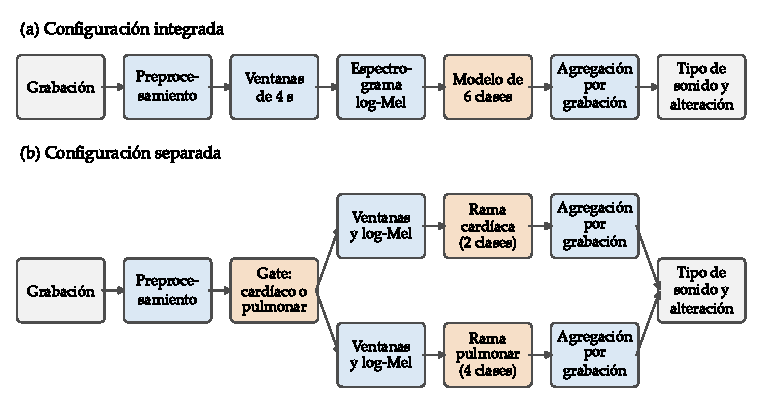
\includegraphics[width=\textwidth]{./Figures/arquitectura.pdf}
	\caption[Configuraciones del sistema]{Diagrama de bloques de las dos configuraciones del
		sistema.}
	\label{fig:arquitectura}
\end{figure}

Ambas configuraciones comparten el preprocesamiento, las particiones de los datos y el
procedimiento de agregación por grabación, y las ramas de la configuración separada reciben las
mismas ventanas que el modelo integrado. Además, las ramas utilizan la misma arquitectura
convolucional y la misma receta de entrenamiento que la red propia de la configuración integrada, y
cada una se entrena con los datos de un solo dominio. De este modo, las dos configuraciones pueden
compararse con una misma arquitectura, y la diferencia de desempeño se debe a la organización del
sistema. La red preentrenada CNN6 se utilizó solo en la configuración integrada, que es la que se
adoptó como sistema final.

Cada configuración tiene ventajas y desventajas. La separada permite que cada rama se especialice
en un solo tipo de sonido, pero los errores del \textit{gate} se propagan: una grabación derivada a
la rama equivocada no puede clasificarse correctamente. La integrada, en cambio, requiere entrenar
y mantener una única red y aprende el tipo de sonido junto con las alteraciones, aunque ambos
dominios comparten la misma representación de entrada y los mismos parámetros. La comparación del
desempeño de ambas configuraciones se presenta en el capítulo \ref{Chapter4}.

%----------------------------------------------------------------------------------------

\section{Pipeline de datos}
\label{sec:pipelineDatos}

En esta sección se describe el recorrido de los datos desde las grabaciones originales hasta las
ventanas con las que se entrenan y evalúan los modelos. Se presentan los criterios con los que se
seleccionaron y etiquetaron las grabaciones, el preprocesamiento de la señal, la segmentación en
ventanas, la partición de los datos y la aumentación aplicada durante el entrenamiento.

\subsection{Selección y etiquetado de las grabaciones}
\label{subsec:seleccion}

Las etiquetas de cada base de datos se llevaron a las seis clases de la subsección
\ref{subsec:clases}. En CirCor DigiScope se utilizaron las 3163 grabaciones de sus 942 pacientes.
Como la presencia de soplo se anota por paciente, junto con los focos en los que se escucha, una
grabación se etiquetó con soplo solo si el paciente presenta un soplo y la grabación corresponde a
uno de esos focos. Las demás grabaciones, incluidas las de los 68 pacientes en los que no pudo
determinarse la presencia de soplo, se consideraron sin soplo. Así, 499 grabaciones de 179
pacientes quedaron en la clase de soplo.

En SPRSound, las etiquetas se obtuvieron a partir de los eventos anotados con su inicio y su fin.
Los eventos de crepitantes finos y gruesos se asignaron a la clase de crepitantes, los de
sibilancias y roncus a la de sibilancias, y los de sibilancia con crepitante a la clase que reúne
ambas alteraciones. El estridor se excluyó, ya que es poco frecuente en la base (74 eventos de 10
pacientes) y no corresponde a ninguna de las clases consideradas. Además, se descartaron las 230
grabaciones anotadas como de mala calidad y 387 grabaciones que no incluyen el número de paciente,
porque no pueden asignarse a una partición sin riesgo de que un mismo paciente quede en
entrenamiento y en prueba. Luego de estos descartes y de los de la subsección
\ref{subsec:ventanas}, quedaron 5920 grabaciones de 854 pacientes.

\subsection{Preprocesamiento de la señal}
\label{subsec:preprocesamiento}

Todas las grabaciones se procesaron con la misma cadena de tres pasos. En primer lugar, se aplicó
un filtro pasa-bajos Butterworth de orden 4 con frecuencia de corte de 2048\,Hz, en ambos sentidos
para no introducir desfasaje, que evita el solapamiento espectral en el paso siguiente. En segundo
lugar, la señal se remuestreó a 4\,kHz. Por último, se normalizó su amplitud para llevar el valor
eficaz (RMS, \textit{Root Mean Square}) a 0,1, de modo que las diferencias de ganancia entre
equipos y grabaciones no influyan en la clasificación. La frecuencia de muestreo de cada grabación
se leyó del propio archivo de audio y no de los metadatos de la base.

La frecuencia de 4\,kHz es la de CirCor DigiScope y permite representar hasta 2\,kHz, un rango que
abarca las alteraciones descritas en la sección \ref{sec:alteraciones}. En SPRSound, grabada a
8\,kHz, se verificó que la energía por encima de 2\,kHz es prácticamente nula en todas las clases,
por lo que el remuestreo no elimina información útil. No se aplicó un filtro pasa-altos, aunque es
habitual en el análisis de sonidos pulmonares para atenuar los ruidos cardíacos, porque en este
sistema eliminaría S1 y S2, que son necesarios para reconocer los sonidos cardíacos.

Para no repetir este procesamiento en cada época de entrenamiento, el audio preprocesado de todas
las grabaciones se almacenó una única vez en un arreglo de enteros de 16 bits, del que luego se
extraen las ventanas.

\subsection{Segmentación en ventanas}
\label{subsec:ventanas}

Cada grabación se dividió en ventanas de 4\,s con un salto de 2\,s, es decir, con una
superposición del 50\,\%. La última ventana se alineó con el final de la grabación, para no perder
el tramo final, y las grabaciones de menos de 4\,s se completaron con ceros. Con esta duración,
cada ventana contiene varios ciclos cardíacos y al menos una parte de un ciclo respiratorio.

Las ventanas cardíacas heredan la etiqueta de su grabación, ya que CirCor DigiScope no indica en
qué momentos se escucha el soplo. En cambio, las ventanas pulmonares se etiquetaron a partir de su
superposición con los eventos anotados en SPRSound, como se ilustra en la figura
\ref{fig:ventanas}. Una ventana se consideró con crepitantes si se superpone al menos 1\,s con un
evento de crepitantes, o con al menos la mitad de su duración, para no perder los eventos más
cortos que ese umbral. El mismo criterio se aplicó a las sibilancias, y las ventanas que cumplen
ambos se asignaron a la clase que reúne las dos alteraciones.

\begin{figure}[htbp]
	\centering
	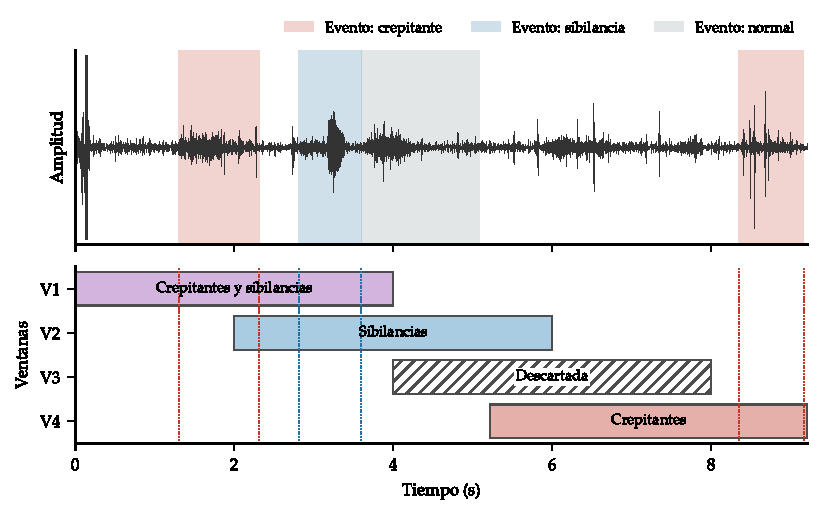
\includegraphics[width=\textwidth]{./Figures/ventanas.pdf}
	\caption[Segmentación y etiquetado de una grabación pulmonar]{Segmentación en ventanas y
		etiquetado de una grabación pulmonar de SPRSound.}
	\label{fig:ventanas}
\end{figure}

Para el entrenamiento se descartaron tres grupos de ventanas pulmonares: las que no se superponen
con ningún evento anotado, ya que se desconoce su contenido; las que tocan un evento de estridor;
y las ventanas normales de grabaciones anormales. Estas últimas se excluyeron porque, en las
grabaciones con alteraciones, los tramos sin anotar presentan una cantidad de transitorios similar
a la de los eventos de crepitantes, lo que sugiere que contienen alteraciones no marcadas. En el
ejemplo de la figura \ref{fig:ventanas}, la segunda ventana se superpone apenas 0,3\,s con el
primer crepitante, por lo que solo recibe la etiqueta de sibilancias, y la tercera se descarta por
ser una ventana normal de una grabación anormal. Estos descartes se aplican solo al conjunto de
entrenamiento. Al evaluar un modelo, cada grabación se procesa con todas sus ventanas, como
ocurriría en el uso real del sistema.

La tabla \ref{tab:distribucionClases} resume la cantidad de ventanas, grabaciones y pacientes de
cada clase. El conjunto está desbalanceado en dos sentidos: dentro de cada dominio predominan las
ventanas normales, y la clase con ambas alteraciones pulmonares reúne apenas 631 ventanas, 46
veces menos que la clase cardíaca normal. El tratamiento de este desbalance se describe junto con
el procedimiento de entrenamiento.

\begin{table}[htbp]
	\centering
	\caption[Distribución de las clases]{Cantidad de ventanas, grabaciones y pacientes de cada
		clase.}
	\label{tab:distribucionClases}
	\small
	\begin{tabular}{l l r r r}
		\toprule
		\textbf{Base} & \textbf{Clase} & \textbf{Ventanas} & \textbf{Grabaciones} & \textbf{Pacientes} \\
		\midrule
		CirCor DigiScope & Cardíaco normal & 29\,111 & 2664 & 831 \\
		 & Soplo & 5412 & 499 & 179 \\
		 & \textit{Total} & 34\,523 & 3163 & 942 \\
		\addlinespace
		SPRSound & Pulmonar normal & 19\,867 & 4218 & 747 \\
		 & Crepitantes & 3931 & 1120 & 240 \\
		 & Sibilancias & 1639 & 512 & 165 \\
		 & Crepitantes y sibilancias & 631 & 214 & 66 \\
		 & \textit{Total} & 26\,068 & 5920 & 854 \\
		\bottomrule
	\end{tabular}
\end{table}

\subsection{Particiones de los datos}
\label{subsec:particiones}

Los modelos se entrenaron y evaluaron con validación cruzada de cinco particiones (\textit{folds})
definidas por paciente, de modo que todas las grabaciones de un paciente quedan siempre en el
mismo subconjunto. Como se mencionó en la sección \ref{sec:estadoArte}, esto evita que el modelo
aproveche características propias de cada paciente o de cada sesión de grabación y sobreestime su
desempeño. En cada partición, un quinto de los pacientes forma el conjunto de prueba, y del resto,
el 15\,\% se reserva para validación y el 85\,\% para entrenamiento. Cada paciente forma parte del
conjunto de prueba en una sola de las cinco particiones, por lo que, al reunir las predicciones de
prueba, se obtiene una predicción para cada grabación de la base, realizada siempre por un modelo
que no vio a ese paciente.

Las particiones se construyeron por separado en cada base, ya que no comparten pacientes, y se
estratificaron para que todas tengan una proporción similar de cada clase. En CirCor DigiScope se
estratificó según si el paciente presenta soplo. En SPRSound, donde un mismo paciente puede tener
grabaciones de varias clases, se estratificó según la clase menos frecuente de cada paciente. La
partición $i$ del sistema es la unión de las particiones $i$ de ambas bases. Todos los modelos y
las dos configuraciones utilizan las mismas cinco particiones, lo que permite comparar sus
resultados paciente por paciente.

\subsection{Aumentación de datos}
\label{subsec:aumentacion}

Durante el entrenamiento se aplicaron dos transformaciones aleatorias a la forma de onda de cada
ventana. La primera modifica la ganancia en un valor elegido entre $-3$ y $+3$\,dB, y la segunda
suma ruido gaussiano con un desvío estándar de 0,005, unos 26\,dB por debajo del nivel de la
señal normalizada. Ambas buscan que el modelo sea robusto a las diferencias de volumen y de ruido
de fondo entre grabaciones y equipos.

En el caso de la CNN6, se agregó además SpecAugment \citep{park2019specaugment} sobre el
espectrograma, la misma técnica utilizada en su preentrenamiento (tabla \ref{tab:cnn6}). En cada
ventana se enmascaran un intervalo de hasta 40 tramas temporales (0,4\,s) y un rango de hasta 6
bandas de frecuencia. Las transformaciones se aplican solo en el entrenamiento: las ventanas de
validación y de prueba se procesan sin modificaciones.

% \definecolor{mygreen}{rgb}{0,0.6,0}
% \definecolor{mygray}{rgb}{0.5,0.5,0.5}
% \definecolor{mymauve}{rgb}{0.58,0,0.82}

% %%%%%%%%%%%%%%%%%%%%%%%%%%%%%%%%%%%%%%%%%%%%%%%%%%%%%%%%%%%%%%%%%%%%%%%%%%%%%
% % parámetros para configurar el formato del código en los entornos lstlisting
% %%%%%%%%%%%%%%%%%%%%%%%%%%%%%%%%%%%%%%%%%%%%%%%%%%%%%%%%%%%%%%%%%%%%%%%%%%%%%
% \lstset{ %
%   backgroundcolor=\color{white},   % choose the background color; you must add \usepackage{color} or \usepackage{xcolor}
%   basicstyle=\footnotesize,        % the size of the fonts that are used for the code
%   breakatwhitespace=false,         % sets if automatic breaks should only happen at whitespace
%   breaklines=true,                 % sets automatic line breaking
%   captionpos=b,                    % sets the caption-position to bottom
%   commentstyle=\color{mygreen},    % comment style
%   deletekeywords={...},            % if you want to delete keywords from the given language
%   %escapeinside={\%*}{*)},          % if you want to add LaTeX within your code
%   %extendedchars=true,              % lets you use non-ASCII characters; for 8-bits encodings only, does not work with UTF-8
%   %frame=single,	                % adds a frame around the code
%   keepspaces=true,                 % keeps spaces in text, useful for keeping indentation of code (possibly needs columns=flexible)
%   keywordstyle=\color{blue},       % keyword style
%   language=[ANSI]C,                % the language of the code
%   %otherkeywords={*,...},           % if you want to add more keywords to the set
%   numbers=left,                    % where to put the line-numbers; possible values are (none, left, right)
%   numbersep=5pt,                   % how far the line-numbers are from the code
%   numberstyle=\tiny\color{mygray}, % the style that is used for the line-numbers
%   rulecolor=\color{black},         % if not set, the frame-color may be changed on line-breaks within not-black text (e.g. comments (green here))
%   showspaces=false,                % show spaces everywhere adding particular underscores; it overrides 'showstringspaces'
%   showstringspaces=false,          % underline spaces within strings only
%   showtabs=false,                  % show tabs within strings adding particular underscores
%   stepnumber=1,                    % the step between two line-numbers. If it's 1, each line will be numbered
%   stringstyle=\color{mymauve},     % string literal style
%   tabsize=2,	                   % sets default tabsize to 2 spaces
%   title=\lstname,                  % show the filename of files included with \lstinputlisting; also try caption instead of title
%   morecomment=[s]{/*}{*/}
% }


% %----------------------------------------------------------------------------------------
% %	SECTION 1
% %----------------------------------------------------------------------------------------
% \section{Análisis del software}
 
% La idea de esta sección es resaltar los problemas encontrados, los criterios utilizados y la justificación de las decisiones que se hayan tomado.

% Se puede agregar código o pseudocódigo dentro de un entorno lstlisting con el siguiente código:

% \begin{verbatim}
% \begin{lstlisting}[caption= "un epígrafe descriptivo"]
% 	las líneas de código irían aquí...
% \end{lstlisting}
% \end{verbatim}

% A modo de ejemplo, se muestra el fragmento de código \ref{cod:vControl}:

% \begin{lstlisting}[label=cod:vControl,caption=Pseudocódigo del lazo principal de control.]  % Start your code-block

% #define MAX_SENSOR_NUMBER 3
% #define MAX_ALARM_NUMBER  6
% #define MAX_ACTUATOR_NUMBER 6

% uint32_t sensorValue[MAX_SENSOR_NUMBER];		
% FunctionalState alarmControl[MAX_ALARM_NUMBER];	//ENABLE or DISABLE
% state_t alarmState[MAX_ALARM_NUMBER];						//ON or OFF
% state_t actuatorState[MAX_ACTUATOR_NUMBER];			//ON or OFF

% void vControl() {

% 	initGlobalVariables();
	
% 	period = 500 ms;
		
% 	while(1) {

% 		ticks = xTaskGetTickCount();
		
% 		updateSensors();
		
% 		updateAlarms();
		
% 		controlActuators();
		
% 		vTaskDelayUntil(&ticks, period);
% 	}
% }
% \end{lstlisting}



